\documentclass{standalone}
\usepackage{pgfplots}
\usetikzlibrary{intersections}
\usepgfplotslibrary{fillbetween}
\pgfplotsset{compat=1.7}

\begin{document}
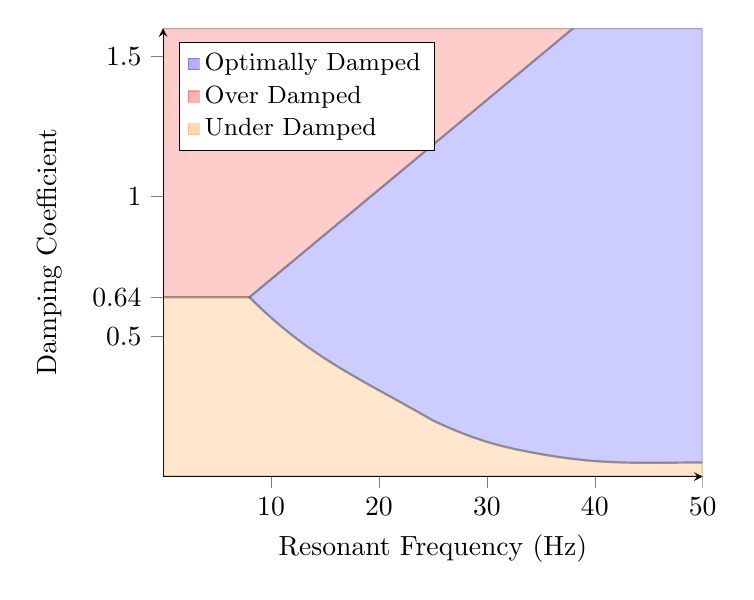
\begin{tikzpicture}


\begin{axis}[
        axis lines=middle,
        grid style={none},
	ymin = 0,
	ymax = 1.6,
	xmin = 0,
	xmax =50,
	 ylabel near ticks,
	xlabel near ticks,
        xlabel=Resonant Frequency (Hz),
        ylabel=Damping Coefficient,
        tick align=outside,
        enlargelimits=false,
	extra y ticks={0.64},
legend pos= north west,
legend style={font=\small, cells={align=left}},
legend cell align={left}]

\addlegendimage{blue, only marks, mark=square*, opacity=0.3}
\addlegendentry{Optimally Damped}
\addlegendimage{red, only marks, mark=square*, opacity=0.3}
\addlegendentry{Over Damped}
\addlegendimage{orange, only marks, mark=square*, opacity=0.3}
\addlegendentry{Under Damped}


\draw[black,thick,fill=red,opacity=0.2] (axis cs: 0,0.64) -- (axis cs: 8, 0.64) -- (axis cs: 38, 1.6) -- (axis cs: 0,1.6) -- cycle;

\draw[black,thick, fill=orange, opacity=0.2] (axis cs: 0,0.64) -- (axis cs: 8, 0.64) to[out=-45, in=150] (axis cs: 25,0.2) to[out=-25, in=170] (axis cs: 35,0.08) to[out=-10, in=180] (axis cs: 50, 0.05) -- (axis cs: 50, 0) -- (axis cs: 0, 0) -- cycle;

\draw[black,thick, fill=blue, opacity=0.2] (axis cs: 8, 0.64) to[out=-45, in=150] (axis cs: 25,0.2) to[out=-25, in=170] (axis cs: 35,0.08) to[out=-10, in=180] (axis cs: 50, 0.05) -- (axis cs: 50, 1.6) -- (axis cs: 38, 1.6) -- cycle;

\end{axis}

\end{tikzpicture} 
\end{document}